%Chapter 6

\renewcommand{\thechapter}{6}

\chapter{Message Aggregation Loop Optimization for Parallel Affine Loops}\label{sec:transformation} 

%\section{Message Aggregation Loop Optimization for Parallel Affine Loops}\label{sec:transformation} 

This chapter describes our method to transform an affine loop that computes on cyclically or block-cyclically distributed data into an equivalent loop that performs message aggregation. As described in Chapter \ref{sec:data_distributions}, our method is not meant for block distributed data. The proposed method is based on modulo unrolling \cite{barua1999maps}, described in Chapter \ref{sec:modulo_unrolling}. Here we describe the method in pseudocode for simplicity and to show that this method is applicable to languages other than Chapel. 

\begin{figure}
\begin{center}
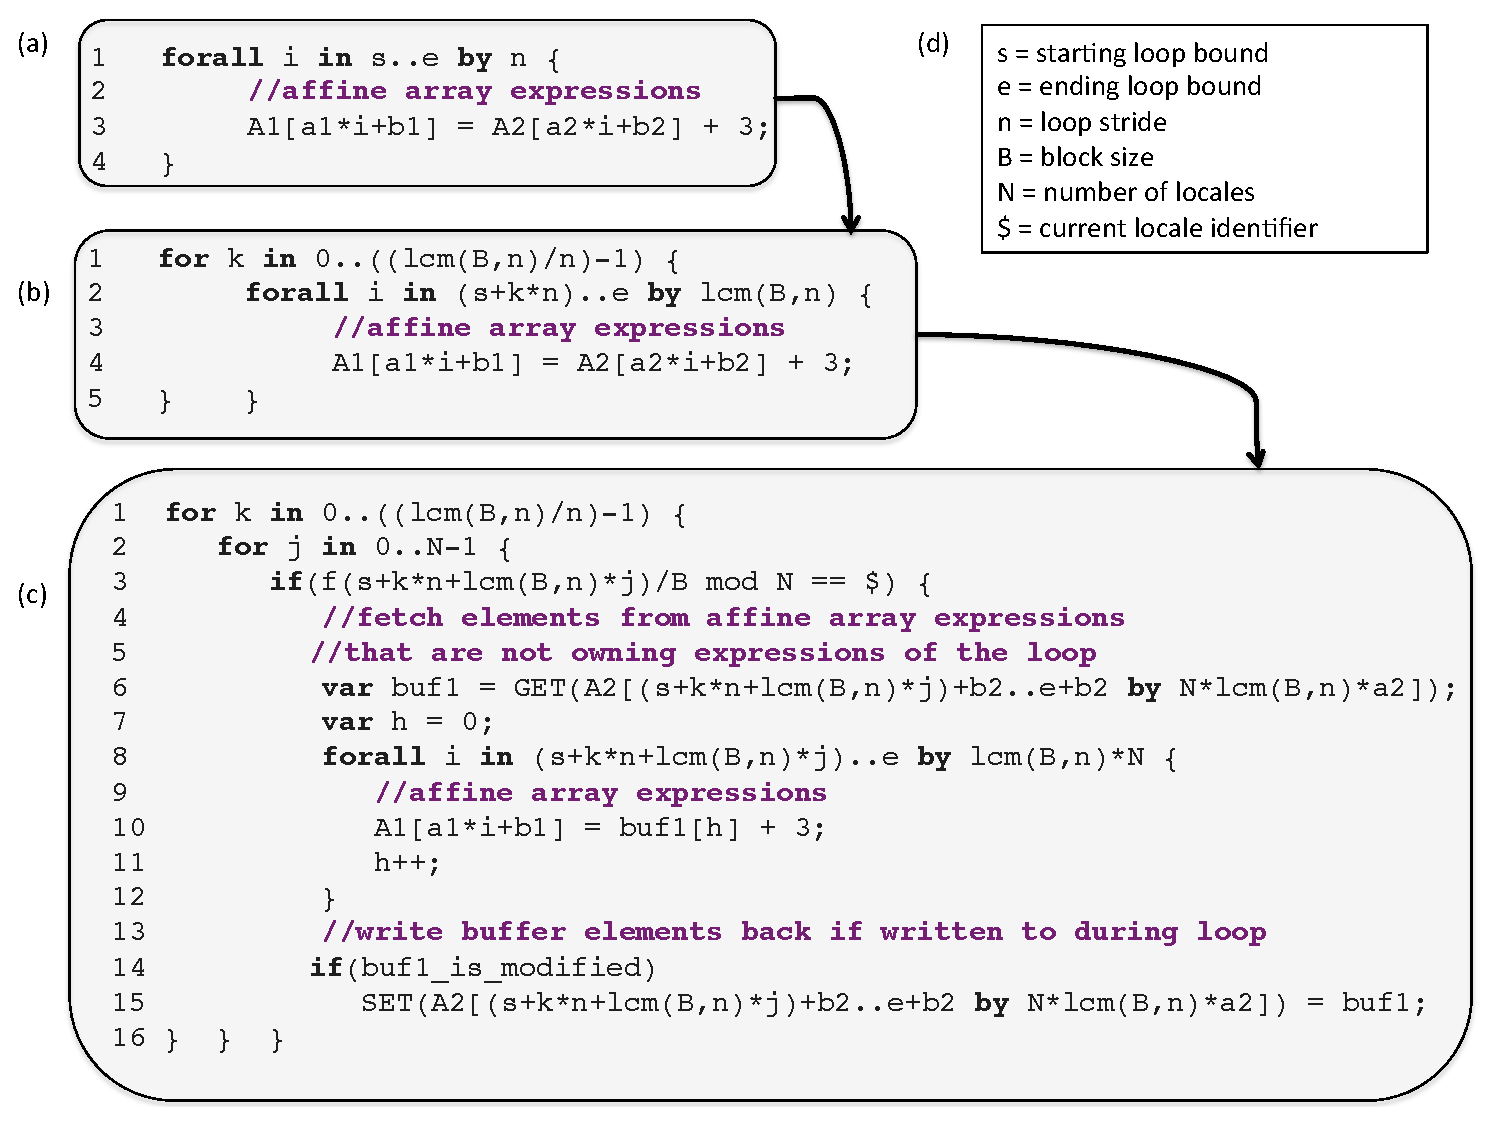
\includegraphics[width=\linewidth]{./Figures/transformations}
\renewcommand{\baselinestretch}{1}
\small\normalsize
\begin{quote}
\caption[Series of transformations to perform modulo unrolling WU]{Steps to transform a parallel affine loop where the data is distributed cyclically or block-cyclically into an equivalent loop that performs message aggregation using modulo unrolling WU. (a) Original distributed parallel loop with two affine array accesses. (b) Loop after Block Cyclic transformation. After this step, the affine array accesses in loops with data distributed block-cyclically will be statically disambiguated. (c) Loop after the owning expression calculation and message aggregation steps. In line 6, remote array elements are communicated to a local buffer before the loop. The affine array access for $A_{2}$ is replaced with an access to the local buffer in line 10. In lines 14-15, elements in the local buffer are written back to the remote locale if they are written to during the loop. (d) Key of symbolic variables used in the transformations in parts a-c. \label{transformations}}
\end{quote}
\end{center}
\end{figure}

\section{Modulo Unrolling Without Unrolling}\label{sec:modulo_unrolling_without_unrolling}

Modulo unrolling increases code size because it unrolls loops by a factor equal to the number of locales (memory banks) on the system. However, we have devised an adaptation called modulo unrolling WU for message passing machines that does not increase code size. To understand it, consider that for parallel machines that use message passing, static disambiguation can be achieved by using the locale identifier without increasing the code size. Conceptually, an affine loop written in source code on a message passing machine where data is distributed cyclically among four locales such as:\newline

\tab{\texttt{\textbf{forall} i \textbf{in} 0..99 \{}}

\tab{\tab{\texttt{A[i] = B[i+2];}}}

\tab{\texttt{\}}}\newline

becomes statically disambiguated using this observation as follows:\newline

\tab{\texttt{\textbf{forall} i \textbf{in} 0..99 \textbf{by} 4 \{}}

\tab{\tab{\texttt{A[i+\$] = B[i+2+\$];}}}

\tab{\texttt{\}}}\newline

where \$ represents the locale identifier. The above is the code that is run on each locale. This transformation is called \textit{modulo unrolling without unrolling (modulo unrolling WU)} since, like modulo unrolling, it can be used for static disambiguation but on message passing machines instead of tiled architectures. Here, no unrolling of the loop is necessary.

Figure \ref{transformations} shows how a generalized affine loop, expressed symbolically, can be transformed by our method in three steps: the Block Cyclic transformation (Figure \ref{transformations}a $\rightarrow$ Figure \ref{transformations}b), the owning expression calculation (described in Chapter \ref{sec:owning_expression_calculation}), and the message aggregation (Figure \ref{transformations}b $\rightarrow$ Figure \ref{transformations}c). 

As shown in Figure \ref{transformations}a, our method takes as its input a parallel \textbf{forall} loop that contains a number of affine array expressions in its loop body. Non-affine expressions are allowed in the loop body, but they are not optimized. The input loop shown in Figure \ref{transformations}a is defined by three explicit parameters: the starting loop bound $s$, the ending loop bound $e$, and the loop stride $n$. The input loop also contains two implicit parameters based on the data distribution. The number of locales the data is distributed over is $N$, and the block size, the number of consecutive array elements allocated to a single locale, is $B$. All five parameters are elements of $\mathbb{N}$. The output of the optimization is an equivalent loop structure that aggregates communication from all of the loop body's remote affine array accesses.

\section{Block Cyclic Transformation}\label{sec:block_cyclic_transformation}

Modulo unrolling as described in \cite{barua1999maps} guarantees static disambiguation for data distributed cyclically but not for block-cyclically distributed data. However, we can think of a Block Cyclic distribution as $B$ adjacent Cyclic distributions, each with a cycle size that is greater than $N$. In order to achieve static disambiguation for the Block Cyclic distribution, we must transform input loops with $B >$ 1 into an equivalent loop with a loop step size that is a multiple of $B$. 

Lines 1 and 2 of Figure \ref{transformations}b show this transformation. We replace the loop step size on line 1 of Figure \ref{transformations}a with the \textit{least common multiple} of $B$ and $n$ in line 2 of Figure \ref{transformations}b. The intuition behind this new step size is that two successive loop iterations accessing the same position within a block will always be separated by a fixed stride length that is a multiple of the block size. To maintain the original meaning of the input loop, an outer \textbf{for} loop is added on line 1 of Figure \ref{transformations}b to handle iterations within each block, and the starting loop bound on line 2 is written in terms of the outer loop variable $k$. After this transformation, all affine array accesses in the loop with be statically disambiguated. This transformation is a variant of the well-known strip mining transformation, which has been used for many other purposes in the literature.

The Cyclic and Block Cyclic distributions are closely related. Any Cyclic distribution can be thought of as a Block Cyclic distribution with $B$ = 1. If we apply the transformation in Figure \ref{transformations}b to a loop with cyclically distributed data, we will end up with the original input loop in Figure \ref{transformations}a, which is already statically disambiguated after applying the transformation described in Chapter \ref{sec:modulo_unrolling_without_unrolling}. 

\section{Owning Expression Calculation}\label{sec:owning_expression_calculation}

There may be many affine array accesses in the input loop, each mapped to a single locale after static disambiguation. For the best communication performance, we must determine the \textit{owning expression} for the loop, which is the most common affine array expression in the loop body. More formally, the owning expression is an affine function $f(i)$, where $i$ is the loop's induction variable, that occurs statically the most number of times in the loop body. We can then use the owning expression to assign loop iterations to locales. Note that there may be instances where affine array expressions are found within control flow statements inside the loop body. Here, we will not know how many times each conditional block will execute at compile time. For these cases, we can use static profiling methods described in \cite{wu1994static} to estimate the occurrences of affine array accesses within conditional blocks in the loop body. 

As an example of how the owning expression is computed and used, consider that there are two affine array accesses in Figure \ref{transformations}b: $A_{1}[a_{1}i+b_{1}]$ and $A_{2}[a_{2}i+b_{2}]$. Each appears once in the loop body, so either expression can be chosen as the owning expression for the loop. For the remainder of Figure \ref{transformations}, we assume that $a_{1}i+b_{1}$ is the owning expression. 

Line 3 of Figure \ref{transformations}c shows symbolically how the owning expression, which is an affine function of the loop induction variable $i$, is used to ensure that loop iterations are assigned to locales such that most of the affine array accesses are local. The argument to the owning expression $f$ in line 3 represents the first loop iteration in each strip-mined portion created in the Block Cyclic transformation. We evaluate the owning expression at this loop iteration. This yields the array index that is most accessed during this loop iteration. The locale where this array index resides should be responsible for handling all iterations in this strip-mined portion because this way most of the loop body's affine array accesses will be local.

\section{Message Aggregation}\label{sec:message_aggregation}

\begin{comment}
This whole writing is very confusing since it is observational, where it simply observes some points about the code. Please write this text to be deductive, meaning you should start with a goal, and then saying how this code meets that goal. (This would also make the text more top down.)

In this case, the goal is to communicate the non-owned accesses, which in this case is the A2[a2*i + b2] access. State that as the goal at the beginning, and then say which portions are remote, and how we generate code to get those portions.
\end{comment}

The final step of the optimization is to communicate the non-owned remote affine array accesses in a single message before the loop. Figure \ref{transformations}c shows this transformation. The loop nest starting on line 2 symbolically represents which loop iterations are assigned to the $N$ locales on the system based on the owning expression calculation (line 3). The array access $A_{2}[a_{2}i+b_{2}]$ is non-owned and may either be entirely remote or entirely local. If entirely remote (as is assumed here), it will require communication. We compute its corresponding remote array slice in line 6 before communicating the entire array slice to a local buffer. Modulo unrolling guarantees that all elements in this array slice are remote with respect to a single locale on the loop iterations that they are used. So, they can be brought to the current locale \$ in one message. Now in lines 8-12, the affine array access $A_{2}[a_{2}i+b_{2}]$ can be replaced with an access to the local buffer. Lines 14-15 handle the case that elements brought over in bulk need to be written back to their remote locale. 

\section{Loops with Multi-Dimensional Array Accesses}\label{sec:multi_dimensional}

The series of transformations described in this chapter and illustrated in Figure \ref{transformations} all apply to one-dimensional arrays indexed by one loop induction variable. These transformations can also be generalized to apply to certain affine array accesses for multi-dimensional arrays. The intuition for this generalization is as follows. The input affine loop now contains $m$ loop induction variables $i_{1}$, $i_{2}$, ... , $i_{m}$. Similarly, there are now $m$ starting loop bounds, ending loop bounds, loop strides, and block sizes. The $p^{th}$ block size is now the number of consecutive array elements allocated to a single locale in dimension $p$ of the array, where $1 \le p \le m$. Each affine array access in the loop body now contains $m$ affine array expressions where expression $p$ is an affine function of $i_{p}$. 

Under these assumptions, the transformations described in this chapter need only be applied to each loop induction variable independently. The owning expression calculation now produces an $m$-tuple of affine array expressions.\footnote{In our adaptation of modulo unrolling WU in Chapel, the Cyclic distribution can apply the optimization to loops with multi-dimensional array accesses, but the Block Cyclic distribution is limited to one-dimensional array accesses because of the current limitations within Chapel's existing Block Cyclic implementation that are outside the scope of this work. } The results we collect in this work consider one-, two-, and three-dimensional array accesses. 